\documentclass{article}
\usepackage{tikz}
\usetikzlibrary{shapes.multipart, positioning, arrows.meta}

\begin{document}
\begin{figure}[htbp]
\centering
\vspace{1cm}
\resizebox{\textwidth}{!}{
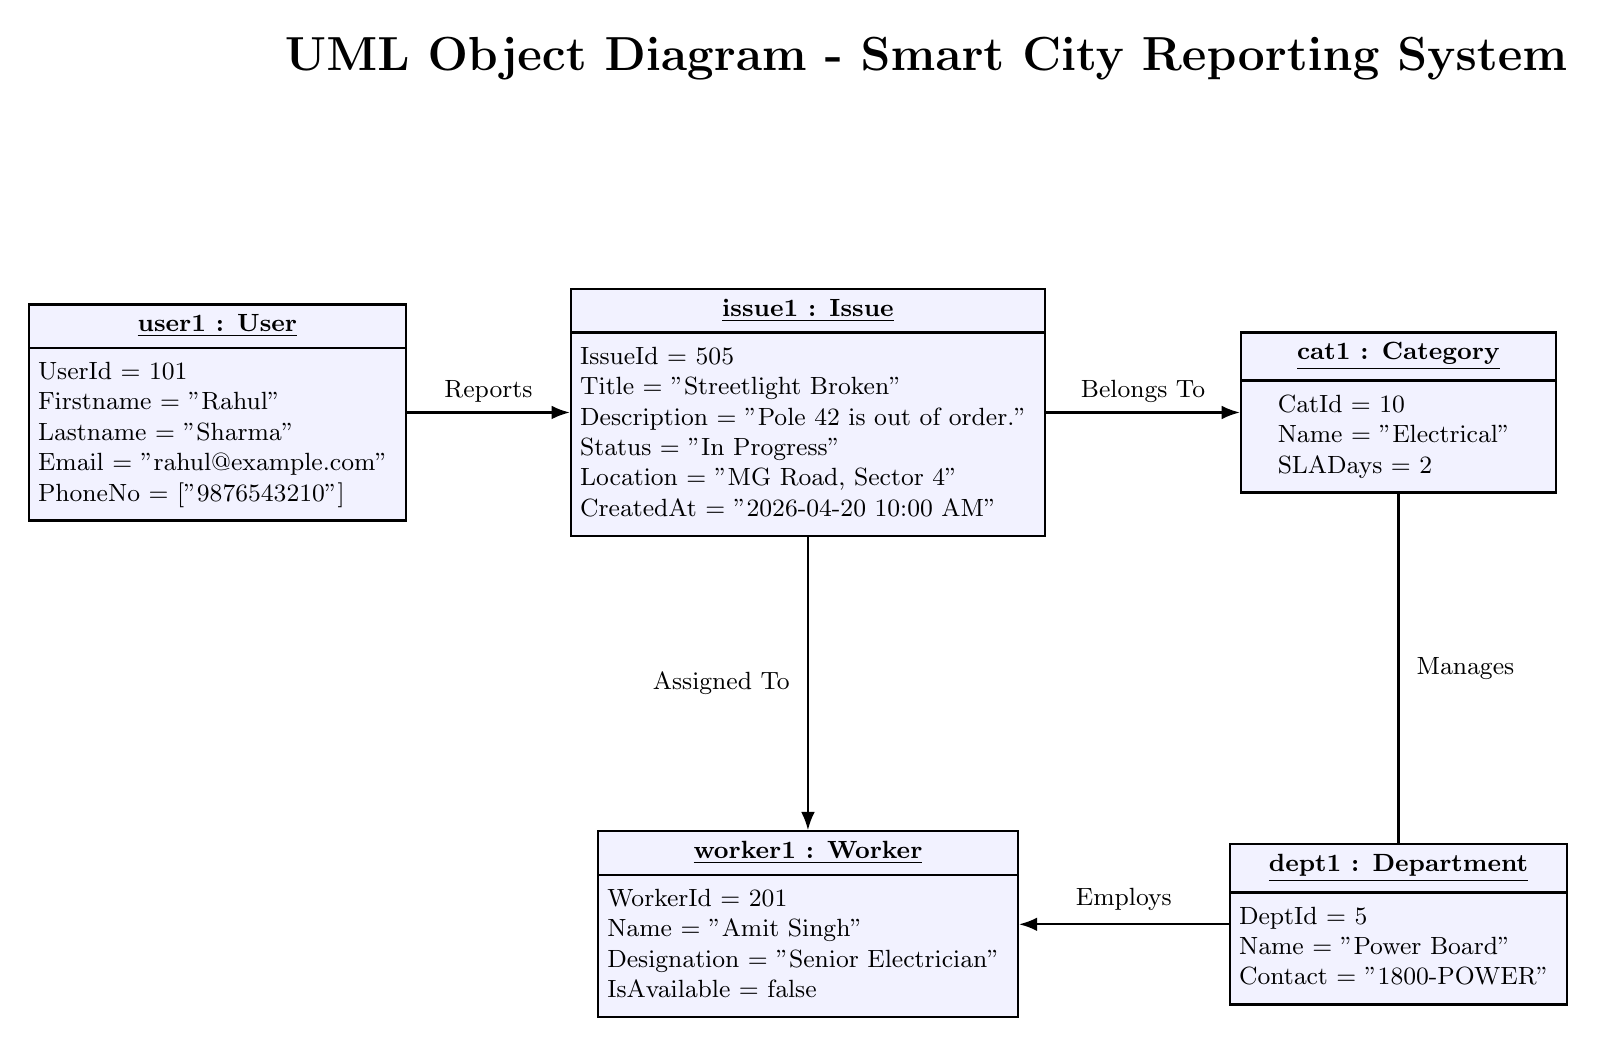
\begin{tikzpicture}[
    >=Latex,
    object/.style={
        draw, rectangle split, rectangle split parts=2,
        minimum width=4cm, align=center, fill=blue!5, thick, font=\small
    }
]

% Title
\node[font=\LARGE\bfseries, align=center] at (1.5, 4.5) {UML Object Diagram - Smart City Reporting System};

% -------------------------
% Object Instances Definition
% -------------------------

% 1. Issue (Center)
\node[object] (issue1) at (0, 0) {
    \underline{\textbf{issue1 : Issue}}
    \nodepart{second}
    \normalfont
    \begin{tabular}{@{}l@{}}
    IssueId = 505 \\
    Title = "Streetlight Broken" \\
    Description = "Pole 42 is out of order." \\
    Status = "In Progress" \\
    Location = "MG Road, Sector 4" \\
    CreatedAt = "2026-04-20 10:00 AM"
    \end{tabular}
};

% 2. User (Left)
\node[object] (user1) at (-7.5, 0) {
    \underline{\textbf{user1 : User}}
    \nodepart{second}
    \normalfont
    \begin{tabular}{@{}l@{}}
    UserId = 101 \\
    Firstname = "Rahul" \\
    Lastname = "Sharma" \\
    Email = "rahul@example.com" \\
    PhoneNo = ["9876543210"]
    \end{tabular}
};

% 3. Category (Right)
\node[object] (cat1) at (7.5, 0) {
    \underline{\textbf{cat1 : Category}}
    \nodepart{second}
    \normalfont
    \begin{tabular}{@{}l@{}}
    CatId = 10 \\
    Name = "Electrical" \\
    SLADays = 2
    \end{tabular}
};

% 4. Worker (Bottom Center)
\node[object] (worker1) at (0, -6.5) {
    \underline{\textbf{worker1 : Worker}}
    \nodepart{second}
    \normalfont
    \begin{tabular}{@{}l@{}}
    WorkerId = 201 \\
    Name = "Amit Singh" \\
    Designation = "Senior Electrician" \\
    IsAvailable = false
    \end{tabular}
};

% 5. Department (Bottom Right)
\node[object] (dept1) at (7.5, -6.5) {
    \underline{\textbf{dept1 : Department}}
    \nodepart{second}
    \normalfont
    \begin{tabular}{@{}l@{}}
    DeptId = 5 \\
    Name = "Power Board" \\
    Contact = "1800-POWER"
    \end{tabular}
};

% -------------------------
% Path Connections (Specific Instance Links)
% Multiplicities are removed in Object Diagrams!
% -------------------------

% issue1 <- user1
\draw[->, thick] (user1.east) -- (issue1.west) 
    node[midway, above, font=\small] {Reports};

% issue1 -> cat1
\draw[->, thick] (issue1.east) -- (cat1.west) 
    node[midway, above, font=\small] {Belongs To};

% issue1 -> worker1 (Vertical, Assigned To)
\draw[->, thick] (issue1.south) -- (worker1.north) 
    node[midway, left=0.1cm, font=\small] {Assigned To};

% dept1 -> worker1
\draw[->, thick] (dept1.west) -- (worker1.east) 
    node[midway, above=0.05cm, font=\small] {Employs};

% dept1 -> cat1 (No Arrow Head)
\draw[-, thick] (dept1.north) -- (cat1.south) 
    node[midway, right=0.1cm, font=\small] {Manages};

\end{tikzpicture}
}
\end{figure}
\end{document}
